%% This is an example first chapter.  You should put chapter/appendix that you
%% write into a separate file, and add a line \include{yourfilename} to
%% main.tex, where `yourfilename.tex' is the name of the chapter/appendix file.
%% You can process specific files by typing their names in at the 
%% \files=
%% prompt when you run the file main.tex through LaTeX.
\chapter{Algorithmic Fabrication: Computational Design, Digital Fabrication and Craft}

\begin{flushright}
\textit{``The mathematician�s patterns, like the painter�s or the poet�s 
must be beautiful; the ideas like the colours or the words, must fit 
together in a harmonious way. Beauty is the first test: there is no 
permanent place in the world for ugly mathematics."
}
G. H. Hardy \cite{hardy}
\end{flushright}


In order to illustrate the creative potential of algorithmic craft, it is useful to examine its contents: computational design , craft and digital fabrication.  Each of these disciplines have separate strengths and limitations when used independently. Through their convergence, new and compelling forms of creation become possible. In computational design, the abstract qualities of computation provide a powerful way of thinking about design. With appropriate programming, a computer can embody any conceivable process \cite{mateas}. Similarly, computational design can be applied to any design domain, be it physical, visual, sonic, or interactive. Although individual applications of computational design often consider material properties that are  relevant to a specific domain, computational design does posses an inherent connection to the material world. Craft on the other hand is rooted in materiality. Craftspeople work in close contact with the physical world and craft artifacts and processes are directly informed by material properties. Digital fabrication provides a connection between the abstraction of computational design and the material domain of craft, by converting digital concepts to physical forms. In the following section I discuss the properties of computational design, digital fabrication and craft in greater detail and demonstrate specific connection points between each medium.

\section{Computational Design}\label{sec:computational_design}
As previously mentioned, computational design can refer to a range of design practices that incorporate programing. My focus in computational design is the process of using computer code to create visual forms and patterns. Because computational design requires the designer to write computer programs, it is possible to mistake the practice of computational design as a technical skill rather than a way of thinking \cite{reas}. Although some degree of technical programing expertise is required, computational design is better represented as a way of applying procedural thinking to a design task.  Rather than producing specific design representations, the designer authors a set of rules that define a system capable of producing many outcomes. Designs are presented in abstract terms, resulting in the potential to create multiple variations that share a set of constraints. One of the challenges of computational design is in authoring guidelines that effectively produce solutions within the desired design space. Presented as an ordered set of instructions, they constitute an algorithim. The ability to read and write and conceive of design algorithms allows for the incorporation of several key properties and methods. These include the following:

\todo{insert work examples by marius watz, sep kamvar, sol deWit, corey archangel and casey reas.... need ideas for female computational designers}


\begin{itemize}
\item \textbf{Precision:} Computation supports high levels of numerical precision with relatively little effort on the part of the designer.
\item \textbf{Visual Complexity:}  Computational design supports the creation and transformation of complex patterns and structures through automation and iteration which allows for the combination and manipulation of large numbers of simple elements in a structured manner. 
\item \textbf{Generativity and randomness:} Computation allows for the programmer to create algorithms which when run, allow for the computer to autonomously produce unique and often unexpected designs.
\item  \textbf{Parameterization:} Computation allows users to specify a set of degrees of freedom and constraints of a model and then adjust the values of the degrees of freedom while maintaining the constraints of the original model.
\item \textbf{Documentation and remixing:} Computationally generated designs are generated by a program, which can be shared with and modified by other designers. Because these programs are often text-based, they also serve as a form of documentation of the design process. 
\end{itemize}	

In combination with these affordances however, computational design also contains a number of unique challenges:
\begin{itemize}
\item \textbf{Formalizing complex problems} As design problems grow in complexity, formalizing the problem in a manner that can be expressed programmatically becomes challenging. Writing an algorithm to generate a visual pattern is simple, however writing a program to incorporate that pattern into the design of an entire garment  is difficult. 
\item \textbf{Creating singularities:} A designer will often choose to deviate from a set pattern or structure at specific points in order to create a special emphasis in that area. Because computational design is governed by a systematized ruleset, the methods of breaking these rules at arbitrary points is are often unclear and tedious to implement. 
\item \textbf{Selecting a final design:}  The systematic approach to computational design gives the designer the ability to produce extremely large numbers of solutions to a single design problem. While this is useful in situations where multiple solutions are required, when a single design must be chosen, the process of deciding on a solution is often difficult and sometimes arbitrary, especially if the decision is based on aesthetic criteria.
\end{itemize}

\section{Digital Fabrication} Although computational design is performed on a computer, the artifacts generated by computational design are not restricted to the screen. Digital fabrication  technology provides the opportunity to translate digital files to physical form. Digital Fabrication is the process of using computer-controlled machines to fabricate objects specified by a digital tool path.  Digital fabrication shares many of the affordances of computational design. In particular, it allows for the creation of physical objects with a high degree of complexity, without formal skill in craft or extensive manual labor. Digital fabrication also allows for the rapid production of small volumes of similar or identical objects. Also, because the artifacts produced through digital fabrication are derived from digital files, anyone with access to the file, and a similar fabrication machine can potentially create a copy of the object, or remix that object with others. 

There are two primary forms of digital-fabrication manufacturing, additive and subtractive. Subtractive processes machine a part by removing pieces from the original material and include tools like laser cutters, computer numerically controlled (CNC) milling machines and vinyl cutters. Additive  processes create a part by incrementally adding successive layers of material. 3D printers are most commonly associated with additive manufacturing, however  ink jet printers and CNC embroidery machines also fit this definition. Although advances in additive technology are occurring at a rapid pace, at this point the material options for 3d printing are limited. Most 3D printers can output objects in a variety of plastics, ceramic and metal composites. Low-end 3D printers are even more constrained, and can only print in one form of ABS plastic. Additive manufacturing is also extremely expensive and often constrained to small build volumes.\todo{reference wood printing 3d printers, other novel 3d printing techniques} 

Unlike most 3D printing technology, subtractive processes can work with a wide range of materials. Laser cutters work well with traditional materials such as  wood, paper and cloth. Vinyl cutters can also be used on cloth and paper, as well as cut vinyl patterns which can be used for screen printing. Milling machines can cut parts from a variety of plastics, foams and wood. In specialized cases these machines can also be modified to function in an additive manner with custom attachments. An example is the adaptation of a 3-Axis ShopBot by machine to function as a threading device to facilitate part of the construction of a Silk Pavilion, created by the Mediated Matter Group at MIT (figure \ref{fig:pavilion} \cite{pavilion}.)  Large-scale subtractive fabrication machines also make it possible to work at a larger scale than additive processes for a lower price.

\begin{center}
\begin{figure}[h!]
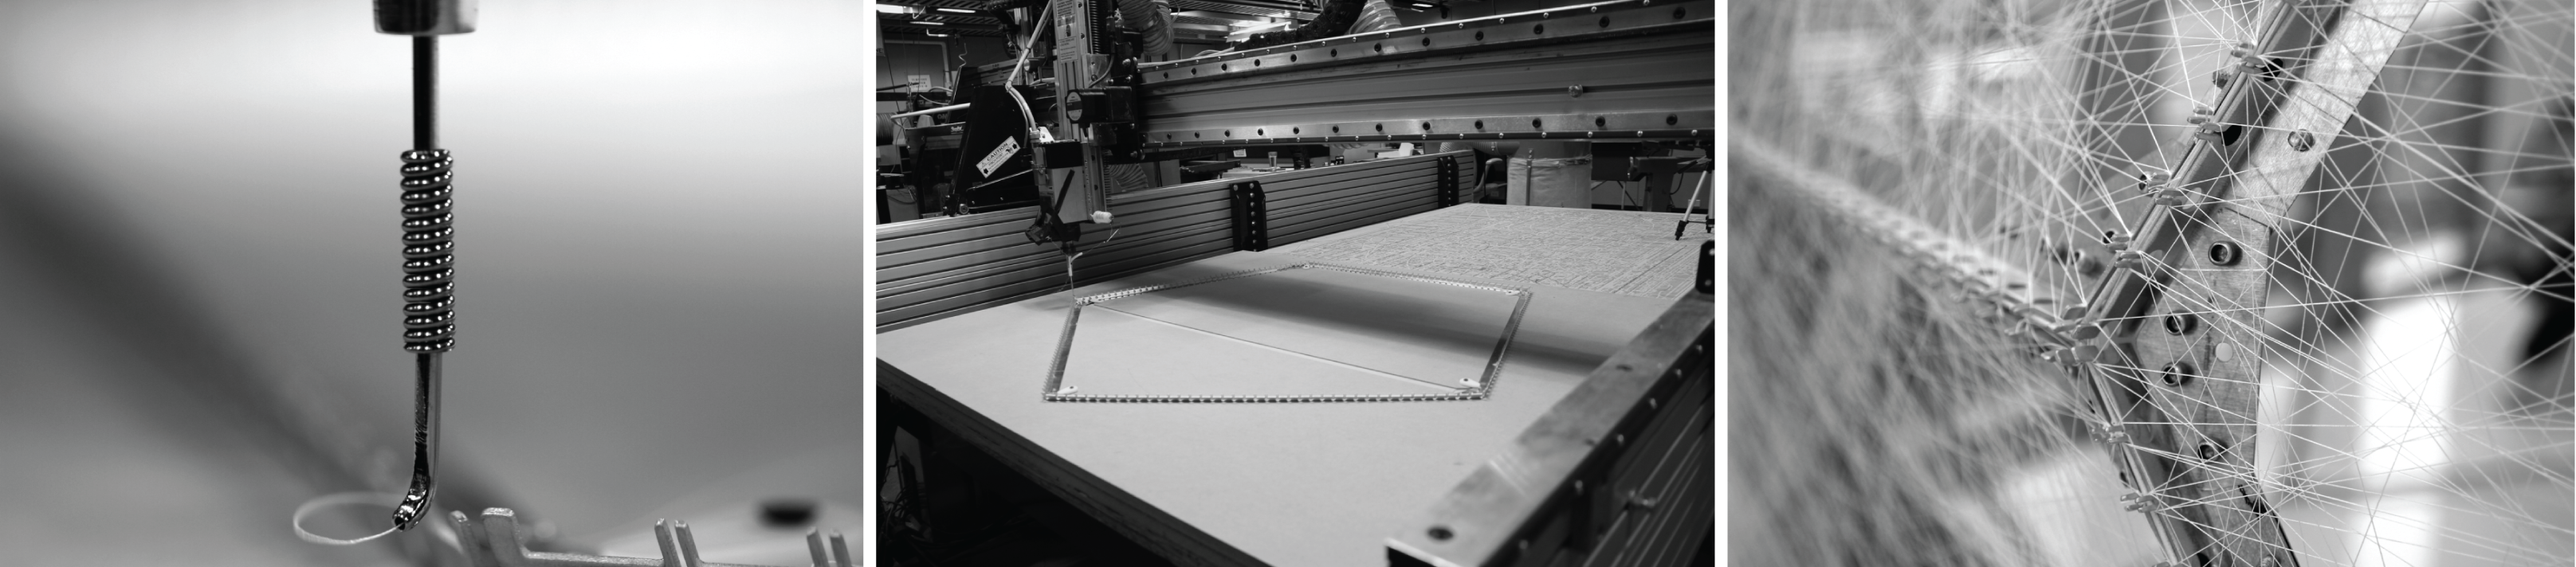
\includegraphics[width=\columnwidth]{images/pavillion_shopbot.png}
\caption{3-axis CNC milling machine adapted as CNC deposition tool using a custom threading tool. (Part of the Silk Pavilion Fabrication process)}
\label{fig:pavilion}
\end{figure}
\end{center}

Widespread access to digital fabrication is growing. Currently, digital fabrication machines are rapidly decreasing in price and increasing in availability \cite{gershenfeld}. The trend of personal fabrication allows individuals and small groups to have access to  sophisticated manufacturing technologies \cite{lipson}. Consumer 3d printers can now be purchased at prices ranging from \$1,000-\$3,500 dollars. Small scale laser cutters and milling machines are available at prices ranging from \$3,000 to \$5,000. \todo{add in citations for prices} In addition, other groups are producing open-source versions of commercial fabrication equipment, like the MTM snap CNC milling machine, the LaserSaur laser cutter and the RepRap 3d printer. Though these devices require additional levels of expertise to assemble, they point to to exciting future developments in the range and accessibility of these machines. Though often dismissed, machines like inkjet printers and craft cnc vinyl cutters also function as personal fabrication devices and are extremely accessible and affordable. 

There are also options for individuals without direct ownership of a fabrication machine. Community hacker spaces like Artisans' Asylum in Cambridge, NYC resistor in New York and Noisebridge in San Francisco, and organizations like the FabLab network provide access to shared digital fabrication facilities.  Online services like Shapeways, Ponoko and SpoonFlower offer on-demand fabrication services to individual consumers for a variety of materials and machining processes. 

The rise of personal fabrication is often viewed as a component of the maker movement \cite{anderson}. The maker subculture is a technology-literate community that is engaged in the production of devices and artifacts in line with the Do-it-yourself or DIY philosophy. While maker culture has a strong technological focus, it also encompasses hobbyist craft techniques and materials. MakerFaire, one of the predominate maker culture events, showcases a range of DIY practice across science, engineering, art, and craft \cite{maker_faire}. In addition, some of the primary tenants of the maker movement correspond to values frequently expressed in craft.

\section{Craft}
The cultural connotations of craft have varied throughout history. Once the primary means of producing functional objects, the role of craft changed following the industrial revolution.  In the face of mechanized production, hand skills became less central, and design, traditionally unified with the role of the artisan emerged as a separate discipline \cite{abstracting_craft}. Despite the emergence of mass production craft  has endured, both as a recreational pursuit, and as set of valued artisanal practices. My personal interest in craft focuses on three specific qualities: materiality, pleasure and craftsmanship.
\begin{itemize}
\item \textbf{Materiality:} One aspect of craft involves the manipulation of physical materials \cite{on_craft}. Working with physical materials requires the use of one's hands, and is often an intuitive process. When we craft, we experience the feel of the paint brush moving across the canvas, the carving knife through a piece of wood, a needle through cloth, or our fingertips pressing into clay. The decisions we make in the craft process are altered by the feel of working with the material. 

\item \textbf{Pleasure:} One of the responses to industrialism was the Arts and Crafts movement, initiated primarily by William Morris, and inspired by the writings of John Ruskin.  
The arts and crafts movement sought to restore the aesthetics and practices of traditional craftsmanship, in response to the negative aesthetic effects and working conditions of industrialism.
Fundamental to the arts and crafts movement was the notion that the act of creating beautiful artifacts with one�s hands was a pleasurable, and essential human experience \cite{abstracting_craft}. This emphasis on pleasure is retained in conceptions of craft today.

\item \textbf{Craftsmanship:} Although not all craft ist functional, many forms of traditional craft, including sewing, pottery, and carpentry can be applied the creation of useful objects. In addition to this functionality, craft often emphasizes the importance of beauty in the form and ornamentation of objects. I use the term craftsmanship to describe the successful unification of aesthetics and utility in a single artifact. 
\end{itemize}

The merging of the properties of craft with computational design and  digital fabrication allows for a creative practice that exhibits the variability and complexity of computation, the precision and repeatability of fabrication and the material and aesthetic concerns of craft. Algorithmic crafting allows individuals use programing and digital fabrication as a means of pleasurable and useful creative expression. In addition, algorithmic craft suggests the incorporation of  the approaches and values of artisans and craftspeople in development of new methods of digital fabrication and computational design tools, paving the way for new forms of innovation in these fields. 

Subtractive fabrication technologies in particular can work with materials often used in traditional forms of craft. For example, laser cutters work well with wood, paper and cloth. Vinyl cutters can also be used on cloth and paper, as well as cut vinyl patterns which can be used for screen printing. Materials like wood, paper and fabric also have the property of being highly mutable following the fabrication process, through sanding, hand-cutting, sewing and folding. 

\todo{Cite Amit Zoran and Peter Schmitt's work here... algorithmic quilt and others?}

\section{Challenges in broad participation in computational design and digital fabrication}
Despite the opportunity for casual, non-professional engagement in computational design and digital fabrication, this domain is largely limited to experts and professionals.  Novice practitioners in this field are confronted with the difficult process of translating their code-based design to a format that is compatible with the target fabrication machine. Furthermore, the challenges involved in designing complex objects from multiple digitally fabricated parts are extremely difficult to tackle for casual users. There are also severe limitations on computational design software for novices capable of supporting digital fabrication. The majority of traditional CAD tools do not contain computational design capabilities intended for novice use. Similarly, novice oriented programing environments lack the functionality to allow the production of designs that are suitable for fabrication. 

There are also significant perceptual barriers to participation. There persists among the general public a  limited perception of the applications of programing. Many people consider programing to be irrelevant to their interests, and therefore lack motivation to pursue what they perceive to be a highly specialized and difficult undertaking \cite{resnick1}. There are also prevailing perceptions of digital fabrication which may hinder casual engagement. Personal fabrication technology is often portrayed as a precursor to the production of replicator-like technology which can instantiate literally anything by building it directly from atoms. This projection of future technology is exciting to think about. This view can also act as a barrier to widespread engagement with existing forms of digital fabrication, by setting up unreal expectations for this technology,or by portraying it as a variation on traditional forms of consumerism. The idea of fabrication as a perfect replication system also eliminates the need or desire for human engagement in the fabrication process, eliminating the entry points for craft. Daniella Rosner describes this view in her research:

\begin{flushright}
 \textit{A central element of these and  other visions of the future is that  craft is done for us: Kitchens tell us what and how to cook, eliminating the creativity and pleasure of  cooking from scratch with what�s on hand; object printers create flawless prototypes, eliminating messily glued-together chipboard and toothpicks. In this new 
world, craft becomes fetish�the proudly displayed collection of vinyl records shelved alongside an iPod and digital files \cite{rosner_craft_vs_design}.}
\end{flushright}

There is also the tendency to trivialize the hobbyist applications of digital fabrication. In the domain of Human Computer Interaction (HCI), researchers often focus on the hedonistic properties technologically oriented DIY practices as opposed to the utility  of the resultant artifacts or their ability to generate profit. Pleasure and self-expression are central components of hobbyist  and craft-oriented computation and digital fabrication, however these qualities do not come at the cost of generating artifacts that are practical, functional, and sellable \cite{tanenbaum}. The trend of separating hobbyist practice as merely fun in contrast to professional practical applications overshadows some of the most interesting practical possibilities that emerge through amateur use of this technology. 


